%! BibTeX Compiler = biber
\documentclass{article}
\usepackage{xcolor}
\definecolor{BLUELINK}{HTML}{0645AD}
\definecolor{DARKBLUELINK}{HTML}{0B0080}
\definecolor{LIGHTBLUELINK}{HTML}{3366BB}
\definecolor{PURPLELINK}{HTML}{663366}
\PassOptionsToPackage{hyphens}{url}
\usepackage[colorlinks=false ]{hyperref}
% for linking between references, figures, TOC, etc in the pdf document
\hypersetup{colorlinks,
linkcolor=DARKBLUELINK,
anchorcolor=DARKBLUELINK,
citecolor=DARKBLUELINK,
filecolor=DARKBLUELINK,
menucolor=DARKBLUELINK,
urlcolor=BLUELINK
} % Color citation links in purple
\PassOptionsToPackage{unicode}{hyperref}
\PassOptionsToPackage{naturalnames}{hyperref}

\usepackage[margin=60pt]{geometry}
\usepackage{amssymb,amsfonts,amsmath,amsthm,mathtools}
\usepackage{lmodern}
\usepackage{bm,bbold}
\usepackage{verbatim}
\usepackage{float}
\usepackage{listings, enumerate, enumitem}
\usepackage[export]{adjustbox}
\usepackage{tabu}
\usepackage{longtable}
\tabulinesep=0.6mm
\newcommand\cellwidth{\TX@col@width}
\usepackage{hhline}
\setlength{\arrayrulewidth}{1.2pt}
\usepackage{multicol,multirow,array}
\usepackage{etoolbox}
\AtBeginEnvironment{tabu}{\footnotesize}
\usepackage{booktabs}

\usepackage{graphicx}
\graphicspath{{artworks/}}
\makeatletter
\def\input@path{{artworks/}}
\makeatother
\pdfstringdefDisableCommands{%
\renewcommand*{\bm}[1]{#1}%
% any other necessary redefinitions
}
\newcommand{\specialcell}[2][c]{%
    \begin{tabular}[#1]{@{}c@{}}#2\end{tabular}}

\usepackage{xfrac, nicefrac}
\usepackage[backend=biber,style=nature]{biblatex}
\addbibresource{codon_models.bib}
\pdfinclusioncopyfonts=1

\begin{document}
\part*{Supplementary materials}
\tableofcontents
 
\pagebreak

\section{Pipeline summary}
\label{subsec:method-summary}

\begin{center}
    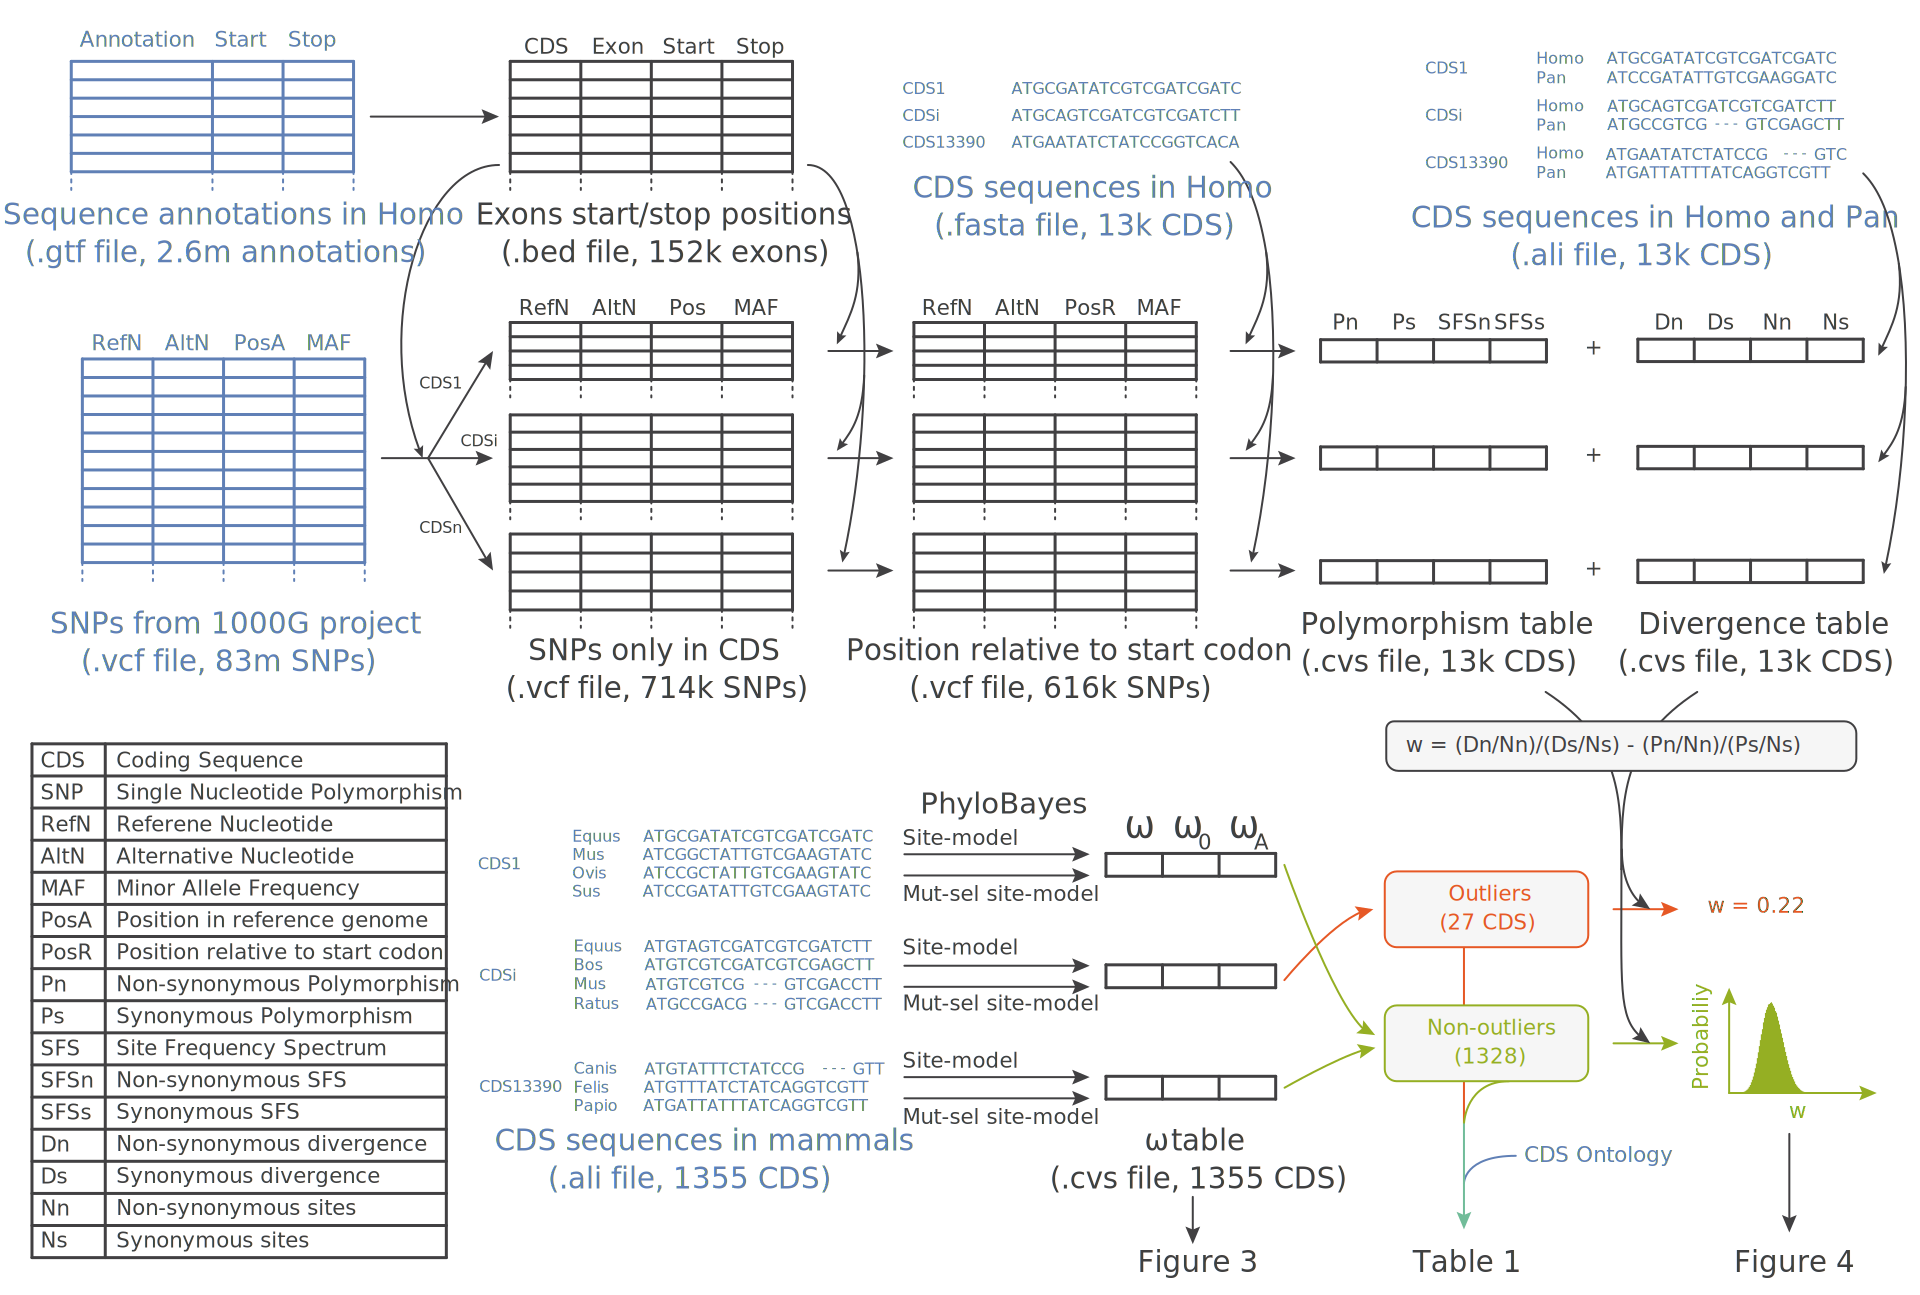
\includegraphics[width=\linewidth]{pipeline}
\end{center}

\pagebreak
\section{Rate of adaptation enrichment with $\alpha=0.005$}
\label{sec:threshold}
For each protein-coding DNA alignment, the Monte-Carlo Markov-Chain (MCMC) is run during $2000$ points using the \href{https://github.com/bayesiancook/bayescode}{BayesCode} software, after a burn-in of $1000$ points.
The mean of $\omega$ and $\omega_{0}$ are computed across the MCMC (after burn-in), as well as the $\bm{99.5}$\% confidence interval ($\alpha=0.005$) for each gene and site, which is more stringent than the $95$\% interval ($\alpha=0.05$) as shown in the main manuscript.
Genes and sites classified under an adaptive regime (in red) are rejecting the nearly-neutral assumption such that a lower bound for the confidence interval of $\omega$ is above the upper bound of the confidence interval of $\omega_{0}$, meaning $\omega > \omega_{0}$.
Genes and sites are classified under a nearly-neutral regime (in green) if the average $\omega$ is within the confidence interval of the $\omega_{0}$, and respectively the average $\omega_{0}$ is also within the confidence interval of  $\omega$, meaning $\omega = \omega_{0}$.
Genes and sites that do not fall in any of these categories are considered unclassified.

\subsection{Scatterplot with $\alpha=0.005$}

\begin{center}
    \begin{minipage}{0.32\linewidth}
        \includegraphics[width=\linewidth, page=1]{scatterplot-gene-MutSel-0.0025}
    \end{minipage}
    \llap{\raisebox{1.2cm}{\scriptsize A\hspace{4.7cm}}}\hfill
    \begin{minipage}{0.32\linewidth}
        \includegraphics[width=\linewidth, page=1]{scatterplot-site-MutSel-0.0025}
    \end{minipage}
    \llap{\raisebox{1.2cm}{\scriptsize B\hspace{4.7cm}}}\hfill
    \begin{minipage}{0.32\linewidth}
        \includegraphics[width=\linewidth, page=1]{scatterplot-site-MutSelExclu-0.0025}
    \end{minipage}
    \llap{\raisebox{1.2cm}{\scriptsize C\hspace{4.7cm}}}\hfill
\end{center}

$\omega$ estimated by the site model against $\omega_{0}$ calculated by the mutation-selection model.
Scatter plot of $14,509$ genes in panel A, with $99.5$\% confidence interval ($\alpha=0.005$).
Density plot of sites in panel B and C.
Genes or sites are then classified whether they detected as adaptive ($\omega > \omega_{0}$ in red) or nearly-neutral ($\omega \simeq \omega_{0}$ in green).
In panel C, the set of sites detected exclusively by mutation-selection codon models have a mean $\omega < 1 $.

\subsection{Mutation-selection codon model at gene level ($\bm{\alpha=0.005}$)}
\begin{center}
    \includegraphics[width=\linewidth]{no_control/gene-MutSel-0.0025-unfolded-MK-wA.pdf}
    \begin{adjustbox}{width = 1\textwidth}
        \begin{tabular}{|l|l|r|r|r|r|r|r|r|}
            \toprule
            Population & Species & \specialcell{$\omega_{\mathrm{A}}$ \\ Adaptive}                & \specialcell{$\left< \omega_{\mathrm{A}} \right>$ \\ Nearly-neutral}                & $\Delta \omega_{\mathrm{A}} $    & $p_{\mathrm{v}}$ & $p_{\mathrm{v}}^{\mathrm{adj}}$ & $\frac{\Delta\omega_{\mathrm{A}}}{\Delta\omega_{\mathrm{A}}^{\mathrm{phy}}}$ & $\pi_{\textrm{S}}$    \\
            \midrule
            Diverse (Equus)                    & Equus caballus          & $ 0.101$ & $-0.024$ & $ 0.125$ & $0.0$ & $\bm{0.0{^*}}$ & $ 1.029$ & $ 0.002$ \\
            Diverse (Canis)                  & Canis familiaris          & $ 0.084$ & $-0.006$ & $ 0.090$ & $0.0$ & $\bm{0.0{^*}}$ & $ 0.722$ & $ 0.004$ \\
            Iran (IRBT)               & Bos taurus        & $ 0.105$ & $ 0.058$ & $ 0.046$ & $ 0.002$    & $\bm{ 0.014{^*}}$    & $ 0.381$ & $ 0.008$ \\
            Uganda (UGBT)                  & Bos taurus        & $ 0.105$ & $ 0.059$ & $ 0.046$ & $ 0.001$ & $\bm{ 0.010{^*}}$ & $ 0.382$ & $ 0.008$ \\
            Australia (AUCH)                    & Capra hircus      & $ 0.088$ & $ 0.013$ & $ 0.075$ & $0.0$    & $\bm{0.0{^*}}$    & $ 0.611$ & $ 0.003$ \\
            France (FRCH)                    & Capra hircus        & $ 0.082$ & $ 0.012$ & $ 0.070$ & $ 0.001$    & $\bm{ 0.010{^*}}$    & $ 0.573$ & $ 0.003$ \\
            Iran (IRCA)                   & Capra aegagrus        & $ 0.103$ & $ 0.031$ & $ 0.073$ & $0.0$    & $\bm{0.0{^*}}$    & $ 0.593$ & $ 0.004$ \\
            Iran (IRCH)                 & Capra hircus        & $ 0.102$ & $ 0.020$ & $ 0.081$ & $0.0$    & $\bm{0.0{^*}}$    & $ 0.662$ & $ 0.004$ \\
            Italy (ITCH)                    & Capra hircus          & $ 0.080$ & $ 0.010$ & $ 0.070$ & $0.0$    & $\bm{0.0{^*}}$    & $ 0.571$ & $ 0.003$ \\
            Morocco (MOCH)                    & Capra hircus     & $ 0.078$ & $ 0.016$ & $ 0.062$ & $0.0$    & $\bm{0.0{^*}}$    & $ 0.504$ & $ 0.004$ \\
            Iran (IROA)                    & Ovis aries         & $ 0.172$ & $ 0.059$ & $ 0.113$ & $0.0$    & $\bm{0.0{^*}}$    & $ 0.919$ & $ 0.007$ \\
            Iran (IROO)                 & Ovis orientalis          & $ 0.166$ & $ 0.062$ & $ 0.104$ & $0.0$    & $\bm{0.0{^*}}$    & $ 0.841$ & $ 0.009$ \\
            Iran (IROV)                 & Ovis vignei          & $ 0.169$ & $ 0.079$ & $ 0.090$ & $0.0$    & $\bm{0.0{^*}}$    & $ 0.726$ & $ 0.005$ \\
            Various (ISGC)                       & Ovis aries & $ 0.167$ & $ 0.062$ & $ 0.105$ & $0.0$    & $\bm{0.0{^*}}$    & $ 0.847$ & $ 0.008$ \\
            Morocco (MOOA) & Ovis aries & $ 0.174$ & $ 0.060$ & $ 0.113$ & $0.0$ & $\bm{0.0{^*}}$ & $ 0.916$ & $ 0.008$ \\
            Barbados                       & Chlorocebus sabaeus & $ 0.096$ & $ 0.003$ & $ 0.093$ & $0.0$    & $\bm{0.0{^*}}$    & $ 0.755$ & $ 0.003$ \\
            Central African Republic (CAR)                         & Chlorocebus sabaeus & $ 0.076$ & $ 0.020$ & $ 0.056$ & $0.0$    & $\bm{0.0{^*}}$    & $ 0.451$ & $ 0.006$ \\
            Ethiopia                          & Chlorocebus sabaeus & $ 0.051$ & $-0.011$ & $ 0.062$ & $0.0$    & $\bm{0.0{^*}}$    & $ 0.504$ & $ 0.005$ \\
            Gambia                          & Chlorocebus sabaeus & $ 0.062$ & $ 0.010$ & $ 0.052$ & $0.0$ & $\bm{0.0{^*}}$        & $ 0.423$ & $ 0.005$ \\
            Kenya              & Chlorocebus sabaeus & $ 0.079$ & $ 0.018$ & $ 0.061$ & $0.0$    & $\bm{0.0{^*}}$ & $ 0.497$ & $ 0.004$ \\
            Nevis               & Chlorocebus sabaeus & $ 0.045$ & $ 0.006$ & $ 0.039$ & $ 0.014$ & $ 0.070~~$ & $ 0.319$ & $ 0.003$ \\
            South Africa (SA)                         & Chlorocebus sabaeus & $ 0.075$ & $ 0.002$ & $ 0.072$ & $0.0$    & $\bm{0.0{^*}}$    & $ 0.587$ & $ 0.006$ \\
            Saint Kitts (SK)                  & Chlorocebus sabaeus        & $ 0.049$ & $ 0.001$ & $ 0.047$ & $ 0.002$ & $\bm{ 0.014{^*}}$        & $ 0.384$ & $ 0.004$ \\
            Zambia        & Chlorocebus sabaeus        & $ 0.077$ & $ 0.004$ & $ 0.073$ & $0.0$ & $\bm{0.0{^*}}$ & $ 0.589$ & $ 0.006$ \\
            African (AFR)               & Homo sapiens        & $ 0.003$ & $-0.033$ & $ 0.036$ & $ 0.071$ & $ 0.174~~$        & $ 0.289$ & $ 0.002$ \\
            Ad Mixed American (AMR)                 & Homo sapiens        & $ 0.004$ & $-0.047$ & $ 0.051$ & $ 0.033$ & $ 0.132~~$        & $ 0.415$ & $ 0.002$ \\
            East Asian (EAS)              & Homo sapiens        & $-0.008$ & $-0.036$ & $ 0.028$ & $ 0.186$ & $ 0.186~~$ & $ 0.227$ & $ 0.002$ \\
            European (EUR)              & Homo sapiens        & $-0.003$ & $-0.049$ & $ 0.046$ & $ 0.058$ & $ 0.174~~$ & $ 0.376$ & $ 0.002$ \\
            South Asian (SAS)              & Homo sapiens        & $ 0.040$ & $-0.045$ & $ 0.084$ & $ 0.001$ & $\bm{ 0.010{^*}}$ & $ 0.688$ & $ 0.002$ \\
            \bottomrule
        \end{tabular}
    \end{adjustbox}
    \newpage
\end{center}

\subsection{Mutation-selection codon model at site level ($\bm{\alpha=0.005}$)}
\begin{center}
    \includegraphics[width=\linewidth]{no_control/site-MutSel-0.0025-unfolded-MK-wA.pdf}
    \begin{adjustbox}{width = 1\textwidth}
        \begin{tabular}{|l|l|r|r|r|r|r|r|r|}
            \toprule
            Population & Species & \specialcell{$\omega_{\mathrm{A}}$ \\ Adaptive}                & \specialcell{$\left< \omega_{\mathrm{A}} \right>$ \\ Nearly-neutral}                & $\Delta \omega_{\mathrm{A}} $    & $p_{\mathrm{v}}$ & $p_{\mathrm{v}}^{\mathrm{adj}}$   & $\frac{\Delta\omega_{\mathrm{A}}}{\Delta\omega_{\mathrm{A}}^{\mathrm{phy}}}$ & $\pi_{\textrm{S}}$    \\
            \midrule
            Diverse (Equus)                    & Equus caballus          & $ 0.646$ & $-0.028$   & $ 0.674$ & $0.0$    & $\bm{0.0{^*}}$ & $ 0.567$ & $ 0.002$ \\
            Diverse (Canis)                  & Canis familiaris          & $ 0.484$ & $-0.003$   & $ 0.487$ & $0.0$    & $\bm{0.0{^*}}$ & $ 0.406$ & $ 0.004$ \\
            Iran (IRBT)               & Bos taurus        & $ 0.495$ & $ 0.072$   & $ 0.423$ & $0.0$ & $\bm{0.0{^*}}$     & $ 0.356$ & $ 0.008$ \\
            Uganda (UGBT)                  & Bos taurus        & $ 0.455$ & $ 0.065$   & $ 0.390$ & $0.0$    & $\bm{0.0{^*}}$ & $ 0.328$ & $ 0.008$ \\
            Australia (AUCH)                    & Capra hircus      & $ 0.143$ & $ 0.001$   & $ 0.142$ & $ 0.043$    & $ 0.258~~$ & $ 0.119$ & $ 0.003$ \\
            France (FRCH)                    & Capra hircus        & $ 0.250$ & $ 0.017$   & $ 0.233$ & $0.0$    & $\bm{0.0{^*}}$ & $ 0.196$ & $ 0.003$ \\
            Iran (IRCA)                   & Capra aegagrus        & $ 0.285$ & $ 0.021$   & $ 0.264$ & $0.0$    & $\bm{0.0{^*}}$ & $ 0.222$ & $ 0.004$ \\
            Iran (IRCH)                 & Capra hircus        & $ 0.288$ & $ 0.012$   & $ 0.276$ & $0.0$    & $\bm{0.0{^*}}$ & $ 0.233$ & $ 0.004$ \\
            Italy (ITCH)                    & Capra hircus          & $ 0.275$ & $ 0.015$   & $ 0.260$ & $0.0$    & $\bm{0.0{^*}}$ & $ 0.219$ & $ 0.003$ \\
            Morocco (MOCH)                    & Capra hircus     & $ 0.299$ & $ 0.012$   & $ 0.287$ & $0.0$    & $\bm{0.0{^*}}$ & $ 0.242$ & $ 0.004$ \\
            Iran (IROA)                    & Ovis aries         & $ 0.349$ & $ 0.070$   & $ 0.279$ & $0.0$    & $\bm{0.0{^*}}$ & $ 0.235$ & $ 0.007$ \\
            Iran (IROO)                 & Ovis orientalis          & $ 0.326$ & $ 0.078$   & $ 0.248$ & $0.0$    & $\bm{0.0{^*}}$ & $ 0.209$ & $ 0.009$ \\
            Iran (IROV)                 & Ovis vignei          & $ 0.279$ & $ 0.106$   & $ 0.174$ & $0.0$    & $\bm{0.0{^*}}$ & $ 0.146$ & $ 0.005$ \\
            Various (ISGC)                       & Ovis aries & $ 0.284$ & $ 0.072$   & $ 0.211$ & $0.0$    & $\bm{0.0{^*}}$ & $ 0.178$ & $ 0.008$ \\
            Morocco (MOOA) & Ovis aries & $ 0.376$ & $ 0.074$   & $ 0.302$ & $0.0$ & $\bm{0.0{^*}}$ & $ 0.254$ & $ 0.008$ \\
            Barbados                       & Chlorocebus sabaeus & $ 0.490$ & $-0.031$   & $ 0.521$ & $0.0$    & $\bm{0.0{^*}}$ & $ 0.438$ & $ 0.003$ \\
            Central African Republic (CAR)                         & Chlorocebus sabaeus & $ 0.467$ & $-0.006$   & $ 0.473$ & $0.0$    & $\bm{0.0{^*}}$ & $ 0.398$ & $ 0.006$ \\
            Ethiopia                          & Chlorocebus sabaeus & $ 0.390$ & $-0.032$ & $ 0.422$ & $0.0$    & $\bm{0.0{^*}}$ & $ 0.355$ & $ 0.005$ \\
            Gambia                          & Chlorocebus sabaeus & $ 0.356$ & $-0.031$   & $ 0.388$ & $0.0$    & $\bm{0.0{^*}}$ & $ 0.326$ & $ 0.005$ \\
            Kenya              & Chlorocebus sabaeus & $ 0.367$ & $-0.00077$   & $ 0.368$ & $0.0$    & $\bm{0.0{^*}}$ & $ 0.310$ & $ 0.004$ \\
            Nevis               & Chlorocebus sabaeus & $ 0.399$ & $-0.045$   & $ 0.444$ & $0.0$    & $\bm{0.0{^*}}$ & $ 0.373$ & $ 0.003$ \\
            South Africa (SA)                         & Chlorocebus sabaeus & $ 0.405$ & $-0.017$   & $ 0.422$ & $0.0$    & $\bm{0.0{^*}}$ & $ 0.355$ & $ 0.006$ \\
            Saint Kitts (SK)                  & Chlorocebus sabaeus        & $ 0.388$ & $-0.048$   & $ 0.436$ & $0.0$ & $\bm{0.0{^*}}$     & $ 0.366$ & $ 0.004$ \\
            Zambia        & Chlorocebus sabaeus        & $ 0.288$ & $-0.028$   & $ 0.315$ & $0.0$ & $\bm{0.0{^*}}$ & $ 0.265$ & $ 0.006$ \\
            African (AFR)               & Homo sapiens        & $ 0.002$ & $-0.034$   & $ 0.036$ & $ 0.423$ & $ 0.794~~$     & $ 0.030$ & $ 0.002$ \\
            Ad Mixed American (AMR)                 & Homo sapiens        & $ 0.086$ & $-0.041$   & $ 0.127$ & $ 0.170$ & $ 0.510~~$     & $ 0.107$ & $ 0.002$ \\
            East Asian (EAS)              & Homo sapiens        & $ 0.111$ & $-0.052$   & $ 0.164$ & $ 0.107$ & $ 0.428~~$     & $ 0.138$ & $ 0.002$ \\
            European (EUR)              & Homo sapiens        & $ 0.167$ & $-0.045$   & $ 0.212$ & $ 0.059$ & $ 0.295~~$     & $ 0.178$ & $ 0.002$ \\
            South Asian (SAS)              & Homo sapiens        & $ 0.017$ & $-0.031$   & $ 0.048$ & $ 0.397$ & $ 0.794~~$     & $ 0.040$ & $ 0.002$ \\
            \bottomrule
        \end{tabular}
    \end{adjustbox}
    \newpage
\end{center}

\subsection{Summary}
\begin{center}
    \includegraphics[width=\linewidth]{no_control/results.pval.pdf}
    \includegraphics[width=\linewidth]{no_control/results.delta_wa.pdf}
\end{center}


\pagebreak
\section{Rate of adaptation enrichment while controlling for $\omega$}
\label{sec:controlling-for-omega}

$\omega$ is controlled to be the same in the nearly-neutral replicate and the adaptive set of genes, such as to alleviate the fact that genes classified as adaptive have a higher $\omega$ than genes classified as nearly-neutral, which could bias our comparison since $\omega_{\mathrm{A}}$ could simply be higher for genes with higher $\omega$.

\begin{center}
    \includegraphics[width=\linewidth]{polymorphism-method-control}
\end{center}

The random sampling is weighted to control for $\omega$ in the set of nearly-neutral genes/sites.
First, a normal distribution is fitted to $\omega$ in both sets, and the probability density is called $f$ for the adaptive set and $g$ for the nearly-neutral set.
Secondly, for each gene/site classified as nearly-neutral the weight is computed as the ratio $f(\omega)/g(\omega)$ for this specific gene/site.
Sampling with this procedure produce a set of genes/sites classified as nearly-neutral with the same $\omega$ on average than the set of adaptive genes/sites.

\subsection{Mutation-selection codon model at gene level ($\bm{\alpha=0.005}$)}
\begin{center}
    \includegraphics[width=\linewidth]{no_control/gene-MutSel-0.0025-unfolded-MK-wA.pdf}
    \begin{adjustbox}{width = 1\textwidth}
        \begin{tabular}{|l|l|r|r|r|r|r|r|r|}
            \toprule
            Population & Species & \specialcell{$\omega_{\mathrm{A}}$ \\ Adaptive}                & \specialcell{$\left< \omega_{\mathrm{A}} \right>$ \\ Nearly-neutral}                & $\Delta \omega_{\mathrm{A}} $    & $p_{\mathrm{v}}$ & $p_{\mathrm{v}}^{\mathrm{adj}}$ & $\frac{\Delta\omega_{\mathrm{A}}}{\Delta\omega_{\mathrm{A}}^{\mathrm{phy}}}$ & $\pi_{\textrm{S}}$    \\
            \midrule
            Diverse (Equus)                    & Equus caballus          & $ 0.101$ & $-0.024$ & $ 0.125$ & $0.0$ & $\bm{0.0{^*}}$ & $ 1.029$ & $ 0.002$ \\
            Diverse (Canis)                  & Canis familiaris          & $ 0.084$ & $-0.006$ & $ 0.090$ & $0.0$ & $\bm{0.0{^*}}$ & $ 0.722$ & $ 0.004$ \\
            Iran (IRBT)               & Bos taurus        & $ 0.105$ & $ 0.058$ & $ 0.046$ & $ 0.002$    & $\bm{ 0.014{^*}}$    & $ 0.381$ & $ 0.008$ \\
            Uganda (UGBT)                  & Bos taurus        & $ 0.105$ & $ 0.059$ & $ 0.046$ & $ 0.001$ & $\bm{ 0.010{^*}}$ & $ 0.382$ & $ 0.008$ \\
            Australia (AUCH)                    & Capra hircus      & $ 0.088$ & $ 0.013$ & $ 0.075$ & $0.0$    & $\bm{0.0{^*}}$    & $ 0.611$ & $ 0.003$ \\
            France (FRCH)                    & Capra hircus        & $ 0.082$ & $ 0.012$ & $ 0.070$ & $ 0.001$    & $\bm{ 0.010{^*}}$    & $ 0.573$ & $ 0.003$ \\
            Iran (IRCA)                   & Capra aegagrus        & $ 0.103$ & $ 0.031$ & $ 0.073$ & $0.0$    & $\bm{0.0{^*}}$    & $ 0.593$ & $ 0.004$ \\
            Iran (IRCH)                 & Capra hircus        & $ 0.102$ & $ 0.020$ & $ 0.081$ & $0.0$    & $\bm{0.0{^*}}$    & $ 0.662$ & $ 0.004$ \\
            Italy (ITCH)                    & Capra hircus          & $ 0.080$ & $ 0.010$ & $ 0.070$ & $0.0$    & $\bm{0.0{^*}}$    & $ 0.571$ & $ 0.003$ \\
            Morocco (MOCH)                    & Capra hircus     & $ 0.078$ & $ 0.016$ & $ 0.062$ & $0.0$    & $\bm{0.0{^*}}$    & $ 0.504$ & $ 0.004$ \\
            Iran (IROA)                    & Ovis aries         & $ 0.172$ & $ 0.059$ & $ 0.113$ & $0.0$    & $\bm{0.0{^*}}$    & $ 0.919$ & $ 0.007$ \\
            Iran (IROO)                 & Ovis orientalis          & $ 0.166$ & $ 0.062$ & $ 0.104$ & $0.0$    & $\bm{0.0{^*}}$    & $ 0.841$ & $ 0.009$ \\
            Iran (IROV)                 & Ovis vignei          & $ 0.169$ & $ 0.079$ & $ 0.090$ & $0.0$    & $\bm{0.0{^*}}$    & $ 0.726$ & $ 0.005$ \\
            Various (ISGC)                       & Ovis aries & $ 0.167$ & $ 0.062$ & $ 0.105$ & $0.0$    & $\bm{0.0{^*}}$    & $ 0.847$ & $ 0.008$ \\
            Morocco (MOOA) & Ovis aries & $ 0.174$ & $ 0.060$ & $ 0.113$ & $0.0$ & $\bm{0.0{^*}}$ & $ 0.916$ & $ 0.008$ \\
            Barbados                       & Chlorocebus sabaeus & $ 0.096$ & $ 0.003$ & $ 0.093$ & $0.0$    & $\bm{0.0{^*}}$    & $ 0.755$ & $ 0.003$ \\
            Central African Republic (CAR)                         & Chlorocebus sabaeus & $ 0.076$ & $ 0.020$ & $ 0.056$ & $0.0$    & $\bm{0.0{^*}}$    & $ 0.451$ & $ 0.006$ \\
            Ethiopia                          & Chlorocebus sabaeus & $ 0.051$ & $-0.011$ & $ 0.062$ & $0.0$    & $\bm{0.0{^*}}$    & $ 0.504$ & $ 0.005$ \\
            Gambia                          & Chlorocebus sabaeus & $ 0.062$ & $ 0.010$ & $ 0.052$ & $0.0$ & $\bm{0.0{^*}}$        & $ 0.423$ & $ 0.005$ \\
            Kenya              & Chlorocebus sabaeus & $ 0.079$ & $ 0.018$ & $ 0.061$ & $0.0$    & $\bm{0.0{^*}}$ & $ 0.497$ & $ 0.004$ \\
            Nevis               & Chlorocebus sabaeus & $ 0.045$ & $ 0.006$ & $ 0.039$ & $ 0.014$ & $ 0.070~~$ & $ 0.319$ & $ 0.003$ \\
            South Africa (SA)                         & Chlorocebus sabaeus & $ 0.075$ & $ 0.002$ & $ 0.072$ & $0.0$    & $\bm{0.0{^*}}$    & $ 0.587$ & $ 0.006$ \\
            Saint Kitts (SK)                  & Chlorocebus sabaeus        & $ 0.049$ & $ 0.001$ & $ 0.047$ & $ 0.002$ & $\bm{ 0.014{^*}}$        & $ 0.384$ & $ 0.004$ \\
            Zambia        & Chlorocebus sabaeus        & $ 0.077$ & $ 0.004$ & $ 0.073$ & $0.0$ & $\bm{0.0{^*}}$ & $ 0.589$ & $ 0.006$ \\
            African (AFR)               & Homo sapiens        & $ 0.003$ & $-0.033$ & $ 0.036$ & $ 0.071$ & $ 0.174~~$        & $ 0.289$ & $ 0.002$ \\
            Ad Mixed American (AMR)                 & Homo sapiens        & $ 0.004$ & $-0.047$ & $ 0.051$ & $ 0.033$ & $ 0.132~~$        & $ 0.415$ & $ 0.002$ \\
            East Asian (EAS)              & Homo sapiens        & $-0.008$ & $-0.036$ & $ 0.028$ & $ 0.186$ & $ 0.186~~$ & $ 0.227$ & $ 0.002$ \\
            European (EUR)              & Homo sapiens        & $-0.003$ & $-0.049$ & $ 0.046$ & $ 0.058$ & $ 0.174~~$ & $ 0.376$ & $ 0.002$ \\
            South Asian (SAS)              & Homo sapiens        & $ 0.040$ & $-0.045$ & $ 0.084$ & $ 0.001$ & $\bm{ 0.010{^*}}$ & $ 0.688$ & $ 0.002$ \\
            \bottomrule
        \end{tabular}
    \end{adjustbox}
    \newpage
\end{center}

\subsection{Mutation-selection codon model at site level ($\bm{\alpha=0.005}$)}
\begin{center}
    \includegraphics[width=\linewidth]{no_control/site-MutSel-0.0025-unfolded-MK-wA.pdf}
    \begin{adjustbox}{width = 1\textwidth}
        \begin{tabular}{|l|l|r|r|r|r|r|r|r|}
            \toprule
            Population & Species & \specialcell{$\omega_{\mathrm{A}}$ \\ Adaptive}                & \specialcell{$\left< \omega_{\mathrm{A}} \right>$ \\ Nearly-neutral}                & $\Delta \omega_{\mathrm{A}} $    & $p_{\mathrm{v}}$ & $p_{\mathrm{v}}^{\mathrm{adj}}$   & $\frac{\Delta\omega_{\mathrm{A}}}{\Delta\omega_{\mathrm{A}}^{\mathrm{phy}}}$ & $\pi_{\textrm{S}}$    \\
            \midrule
            Diverse (Equus)                    & Equus caballus          & $ 0.646$ & $-0.028$   & $ 0.674$ & $0.0$    & $\bm{0.0{^*}}$ & $ 0.567$ & $ 0.002$ \\
            Diverse (Canis)                  & Canis familiaris          & $ 0.484$ & $-0.003$   & $ 0.487$ & $0.0$    & $\bm{0.0{^*}}$ & $ 0.406$ & $ 0.004$ \\
            Iran (IRBT)               & Bos taurus        & $ 0.495$ & $ 0.072$   & $ 0.423$ & $0.0$ & $\bm{0.0{^*}}$     & $ 0.356$ & $ 0.008$ \\
            Uganda (UGBT)                  & Bos taurus        & $ 0.455$ & $ 0.065$   & $ 0.390$ & $0.0$    & $\bm{0.0{^*}}$ & $ 0.328$ & $ 0.008$ \\
            Australia (AUCH)                    & Capra hircus      & $ 0.143$ & $ 0.001$   & $ 0.142$ & $ 0.043$    & $ 0.258~~$ & $ 0.119$ & $ 0.003$ \\
            France (FRCH)                    & Capra hircus        & $ 0.250$ & $ 0.017$   & $ 0.233$ & $0.0$    & $\bm{0.0{^*}}$ & $ 0.196$ & $ 0.003$ \\
            Iran (IRCA)                   & Capra aegagrus        & $ 0.285$ & $ 0.021$   & $ 0.264$ & $0.0$    & $\bm{0.0{^*}}$ & $ 0.222$ & $ 0.004$ \\
            Iran (IRCH)                 & Capra hircus        & $ 0.288$ & $ 0.012$   & $ 0.276$ & $0.0$    & $\bm{0.0{^*}}$ & $ 0.233$ & $ 0.004$ \\
            Italy (ITCH)                    & Capra hircus          & $ 0.275$ & $ 0.015$   & $ 0.260$ & $0.0$    & $\bm{0.0{^*}}$ & $ 0.219$ & $ 0.003$ \\
            Morocco (MOCH)                    & Capra hircus     & $ 0.299$ & $ 0.012$   & $ 0.287$ & $0.0$    & $\bm{0.0{^*}}$ & $ 0.242$ & $ 0.004$ \\
            Iran (IROA)                    & Ovis aries         & $ 0.349$ & $ 0.070$   & $ 0.279$ & $0.0$    & $\bm{0.0{^*}}$ & $ 0.235$ & $ 0.007$ \\
            Iran (IROO)                 & Ovis orientalis          & $ 0.326$ & $ 0.078$   & $ 0.248$ & $0.0$    & $\bm{0.0{^*}}$ & $ 0.209$ & $ 0.009$ \\
            Iran (IROV)                 & Ovis vignei          & $ 0.279$ & $ 0.106$   & $ 0.174$ & $0.0$    & $\bm{0.0{^*}}$ & $ 0.146$ & $ 0.005$ \\
            Various (ISGC)                       & Ovis aries & $ 0.284$ & $ 0.072$   & $ 0.211$ & $0.0$    & $\bm{0.0{^*}}$ & $ 0.178$ & $ 0.008$ \\
            Morocco (MOOA) & Ovis aries & $ 0.376$ & $ 0.074$   & $ 0.302$ & $0.0$ & $\bm{0.0{^*}}$ & $ 0.254$ & $ 0.008$ \\
            Barbados                       & Chlorocebus sabaeus & $ 0.490$ & $-0.031$   & $ 0.521$ & $0.0$    & $\bm{0.0{^*}}$ & $ 0.438$ & $ 0.003$ \\
            Central African Republic (CAR)                         & Chlorocebus sabaeus & $ 0.467$ & $-0.006$   & $ 0.473$ & $0.0$    & $\bm{0.0{^*}}$ & $ 0.398$ & $ 0.006$ \\
            Ethiopia                          & Chlorocebus sabaeus & $ 0.390$ & $-0.032$ & $ 0.422$ & $0.0$    & $\bm{0.0{^*}}$ & $ 0.355$ & $ 0.005$ \\
            Gambia                          & Chlorocebus sabaeus & $ 0.356$ & $-0.031$   & $ 0.388$ & $0.0$    & $\bm{0.0{^*}}$ & $ 0.326$ & $ 0.005$ \\
            Kenya              & Chlorocebus sabaeus & $ 0.367$ & $-0.00077$   & $ 0.368$ & $0.0$    & $\bm{0.0{^*}}$ & $ 0.310$ & $ 0.004$ \\
            Nevis               & Chlorocebus sabaeus & $ 0.399$ & $-0.045$   & $ 0.444$ & $0.0$    & $\bm{0.0{^*}}$ & $ 0.373$ & $ 0.003$ \\
            South Africa (SA)                         & Chlorocebus sabaeus & $ 0.405$ & $-0.017$   & $ 0.422$ & $0.0$    & $\bm{0.0{^*}}$ & $ 0.355$ & $ 0.006$ \\
            Saint Kitts (SK)                  & Chlorocebus sabaeus        & $ 0.388$ & $-0.048$   & $ 0.436$ & $0.0$ & $\bm{0.0{^*}}$     & $ 0.366$ & $ 0.004$ \\
            Zambia        & Chlorocebus sabaeus        & $ 0.288$ & $-0.028$   & $ 0.315$ & $0.0$ & $\bm{0.0{^*}}$ & $ 0.265$ & $ 0.006$ \\
            African (AFR)               & Homo sapiens        & $ 0.002$ & $-0.034$   & $ 0.036$ & $ 0.423$ & $ 0.794~~$     & $ 0.030$ & $ 0.002$ \\
            Ad Mixed American (AMR)                 & Homo sapiens        & $ 0.086$ & $-0.041$   & $ 0.127$ & $ 0.170$ & $ 0.510~~$     & $ 0.107$ & $ 0.002$ \\
            East Asian (EAS)              & Homo sapiens        & $ 0.111$ & $-0.052$   & $ 0.164$ & $ 0.107$ & $ 0.428~~$     & $ 0.138$ & $ 0.002$ \\
            European (EUR)              & Homo sapiens        & $ 0.167$ & $-0.045$   & $ 0.212$ & $ 0.059$ & $ 0.295~~$     & $ 0.178$ & $ 0.002$ \\
            South Asian (SAS)              & Homo sapiens        & $ 0.017$ & $-0.031$   & $ 0.048$ & $ 0.397$ & $ 0.794~~$     & $ 0.040$ & $ 0.002$ \\
            \bottomrule
        \end{tabular}
    \end{adjustbox}
    \newpage
\end{center}

\subsection{Summary}
\begin{center}
    \includegraphics[width=\linewidth]{no_control/results.pval.pdf}
    \includegraphics[width=\linewidth]{no_control/results.delta_wa.pdf}
\end{center}


\pagebreak
\section{Gene ontology enrichment at site level}
\label{sec:gene-ontology-enrichment}

Genes are considered under adaptation if at least one site has been detected under adaptation (unilateral test with $\alpha=0.0025$ for each site).

\subsection{$\omega$-based codon model}
\label{subsec:w-based-codon-method}
\normalfont
Sites are classified under an adaptive regime if the lower bound for the confidence interval of $\omega$ is above 1.
925 tests performed with 426 genes detected with $\omega$-based codon models, and with 5499 genes as control.
\begin{longtable}{|l|r|r|r|r|r|}
\toprule
                                     Gene Ontology & $n_{\mathrm{Observed}}$ & $n_{\mathrm{Expected}}$ & Odds ratio &     $p_{\mathrm{v}}$ &     $p_{\mathrm{v-adjusted}}$ \\
\midrule
\endhead
\midrule
\multicolumn{6}{r}{{Continued on next page}} \\
\midrule
\endfoot

\bottomrule
\endlastfoot
                               blood microparticle &                      17 &                   1.568 &       10.8 & 1.9$\times 10^{-10}$ &  1.7$\times 10^{-7}$$\bm{^*}$ \\
                             complement activation &                      11 &                   0.302 &       36.4 & 2.5$\times 10^{-10}$ &  2.3$\times 10^{-7}$$\bm{^*}$ \\
                             immune system process &                      35 &                   8.426 &      4.154 & 2.6$\times 10^{-10}$ &  2.4$\times 10^{-7}$$\bm{^*}$ \\
                            innate immune response &                      32 &                   7.521 &      4.255 & 8.6$\times 10^{-10}$ &  7.9$\times 10^{-7}$$\bm{^*}$ \\
               regulation of complement activation &                      12 &                   0.603 &       19.9 &  1.2$\times 10^{-9}$ &  1.1$\times 10^{-6}$$\bm{^*}$ \\
                            platelet degranulation &                      16 &                   2.324 &      6.883 &  7.3$\times 10^{-8}$ &  6.7$\times 10^{-5}$$\bm{^*}$ \\
                               extracellular space &                      64 &                    28.8 &      2.224 &  2.1$\times 10^{-7}$ &              0.00019$\bm{^*}$ \\
                              extracellular region &                      86 &                    43.4 &      1.980 &    3$\times 10^{-7}$ &              0.00028$\bm{^*}$ \\
                  external side of plasma membrane &                      19 &                   3.885 &      4.890 &  3.3$\times 10^{-7}$ &              0.00031$\bm{^*}$ \\
                                        hemostasis &                      11 &                   1.211 &      9.083 &  1.1$\times 10^{-6}$ &              0.00097$\bm{^*}$ \\
                             complement activation &                       7 &                   0.305 &       23.0 &  2.4$\times 10^{-6}$ &                0.002$\bm{^*}$ \\
                               leukocyte migration &                      15 &                   2.860 &      5.245 &  2.7$\times 10^{-6}$ &                0.002$\bm{^*}$ \\
                                   immune response &                      21 &                   5.752 &      3.651 &  4.3$\times 10^{-6}$ &                0.004$\bm{^*}$ \\
                             extracellular exosome &                      94 &                    52.7 &      1.785 &  4.6$\times 10^{-6}$ &                0.004$\bm{^*}$ \\
                           lipid metabolic process &                      32 &                    11.9 &      2.693 &  5.6$\times 10^{-6}$ &                0.005$\bm{^*}$ \\
                      platelet alpha granule lumen &                      10 &                   1.290 &      7.752 &  9.2$\times 10^{-6}$ &                0.008$\bm{^*}$ \\
                         defense response to virus &                      13 &                   2.417 &      5.378 &  9.9$\times 10^{-6}$ &                0.009$\bm{^*}$ \\
                    integral component of membrane &                     164 &                   104.4 &      1.571 &  1.2$\times 10^{-5}$ &                0.011$\bm{^*}$ \\
                                 receptor activity &                      18 &                   4.956 &      3.632 &  2.1$\times 10^{-5}$ &                0.019$\bm{^*}$ \\
                                          synapsis &                       7 &                   0.534 &       13.1 &  2.1$\times 10^{-5}$ &                0.019$\bm{^*}$ \\
                                      fibrinolysis &                       6 &                   0.306 &       19.6 &  2.2$\times 10^{-5}$ &                0.020$\bm{^*}$ \\
                                chemokine activity &                       5 &                   0.153 &       32.6 &  3.5$\times 10^{-5}$ &                0.032$\bm{^*}$ \\
             integral component of plasma membrane &                      57 &                    30.0 &      1.902 &  4.2$\times 10^{-5}$ &                0.038$\bm{^*}$ \\
                                      cell surface &                      29 &                    11.7 &      2.485 &  5.1$\times 10^{-5}$ &                0.046$\bm{^*}$ \\
                        dynein light chain binding &                       5 &                   0.230 &       21.8 &  8.8$\times 10^{-5}$ &                       0.079~~ \\
                            apical plasma membrane &                      21 &                   7.349 &      2.858 &  9.4$\times 10^{-5}$ &                       0.085~~ \\
                                  receptor binding &                      24 &                   9.121 &      2.631 &  9.8$\times 10^{-5}$ &                       0.088~~ \\
           cell surface receptor signaling pathway &                      18 &                   6.023 &      2.988 &              0.00018 &                       0.157~~ \\
                serine-type endopeptidase activity &                      13 &                   3.408 &      3.815 &              0.00018 &                       0.163~~ \\
                     receptor-mediated endocytosis &                      12 &                   3.110 &      3.859 &              0.00029 &                       0.259~~ \\
                      condensed nuclear chromosome &                       7 &                   0.993 &      7.050 &              0.00032 &                       0.288~~ \\
                     regulation of immune response &                       8 &                   1.373 &      5.828 &              0.00033 &                       0.294~~ \\
                             extracellular vesicle &                       8 &                   1.373 &      5.828 &              0.00033 &                       0.294~~ \\
                    heterotypic cell-cell adhesion &                       5 &                   0.383 &       13.0 &              0.00035 &                       0.312~~ \\
                                fibrinogen complex &                       4 &                   0.154 &       26.1 &              0.00035 &                       0.313~~ \\
          negative regulation of blood coagulation &                       4 &                   0.154 &       26.1 &              0.00035 &                       0.313~~ \\
                              cell-matrix adhesion &                      10 &                   2.282 &      4.382 &               0.0004 &                       0.352~~ \\
                           virus receptor activity &                       8 &                   1.449 &      5.520 &              0.00044 &                       0.389~~ \\
               positive regulation of angiogenesis &                      11 &                   2.811 &      3.913 &              0.00046 &                       0.410~~ \\
                                   plasma membrane &                     138 &                    95.5 &      1.446 &              0.00049 &                       0.438~~ \\
                                            cilium &                      17 &                   6.191 &      2.746 &               0.0006 &                       0.532~~ \\
                 positive regulation of exocytosis &                       5 &                   0.460 &       10.9 &               0.0006 &                       0.533~~ \\
                                     cell adhesion &                      27 &                    12.7 &      2.134 &              0.00073 &                       0.643~~ \\
                               receptor clustering &                       4 &                   0.230 &       17.4 &              0.00077 &                       0.683~~ \\
                    natural killer cell activation &                       4 &                   0.230 &       17.4 &              0.00077 &                       0.683~~ \\
         low-density lipoprotein receptor activity &                       4 &                   0.230 &       17.4 &              0.00077 &                       0.683~~ \\
 positive regulation of heterotypic cell-cell a... &                       4 &                   0.230 &       17.4 &              0.00077 &                       0.683~~ \\
                            plasminogen activation &                       4 &                   0.230 &       17.4 &              0.00077 &                       0.683~~ \\
                                 blood coagulation &                      13 &                   4.096 &      3.174 &               0.0008 &                       0.706~~ \\
                                retina homeostasis &                       5 &                   0.537 &      9.318 &              0.00097 &                       0.852~~ \\
  positive regulation of interleukin-12 production &                       5 &                   0.537 &      9.318 &              0.00097 &                       0.852~~ \\
                                        peroxisome &                      10 &                   2.665 &      3.753 &                0.001 &                       0.942~~ \\
                      fatty acid metabolic process &                      12 &                   3.722 &      3.224 &                0.001 &                       0.976~~ \\
\end{longtable}


\subsection{Mutation-selection codon model}
\label{subsec:mutation-selection-codon-method}
\normalfont
Sites are classified under an adaptive regime if the lower bound for the confidence interval of $\omega$ is above the upper bound of the confidence interval of $\omega_{0}$, meaning $\omega > \omega_{0}$.
2617 tests performed with 1793 genes detected with mutation-selection codon models, and with 4132 genes as control.
\begin{longtable}{|l|r|r|r|r|r|}
\toprule
                                     Gene Ontology & $n_{\mathrm{Observed}}$ & $n_{\mathrm{Expected}}$ & Odds ratio &     $p_{\mathrm{v}}$ &     $p_{\mathrm{v-adjusted}}$ \\
\midrule
\endhead
\midrule
\multicolumn{6}{r}{{Continued on next page}} \\
\midrule
\endfoot

\bottomrule
\endlastfoot
                              extracellular region &                     296 &                   166.2 &      1.781 & 2.9$\times 10^{-12}$ &  7.6$\times 10^{-9}$$\bm{^*}$ \\
                           lipid metabolic process &                     104 &                    37.2 &      2.797 & 3.2$\times 10^{-12}$ &  8.5$\times 10^{-9}$$\bm{^*}$ \\
                             extracellular exosome &                     343 &                   201.4 &      1.703 & 4.6$\times 10^{-12}$ &  1.2$\times 10^{-8}$$\bm{^*}$ \\
                      fatty acid metabolic process &                      44 &                   7.226 &      6.090 & 1.6$\times 10^{-11}$ &  4.1$\times 10^{-8}$$\bm{^*}$ \\
                             immune system process &                      85 &                    27.7 &      3.066 & 1.6$\times 10^{-11}$ &  4.1$\times 10^{-8}$$\bm{^*}$ \\
                            apical plasma membrane &                      70 &                    20.7 &      3.385 & 6.7$\times 10^{-11}$ &  1.7$\times 10^{-7}$$\bm{^*}$ \\
                                   plasma membrane &                     554 &                   371.4 &      1.492 & 1.9$\times 10^{-10}$ &  5.1$\times 10^{-7}$$\bm{^*}$ \\
                            innate immune response &                      73 &                    26.2 &      2.786 &  4.9$\times 10^{-9}$ &  1.3$\times 10^{-5}$$\bm{^*}$ \\
                               extracellular space &                     198 &                   112.0 &      1.769 &  7.1$\times 10^{-9}$ &  1.9$\times 10^{-5}$$\bm{^*}$ \\
             integral component of plasma membrane &                     198 &                   112.4 &      1.762 &  8.8$\times 10^{-9}$ &  2.3$\times 10^{-5}$$\bm{^*}$ \\
                               blood microparticle &                      28 &                   4.282 &      6.539 &    4$\times 10^{-8}$ &               0.0001$\bm{^*}$ \\
                              cell-matrix adhesion &                      29 &                   4.709 &      6.159 &  4.1$\times 10^{-8}$ &              0.00011$\bm{^*}$ \\
               regulation of complement activation &                      18 &                   0.860 &       20.9 &  4.1$\times 10^{-8}$ &              0.00011$\bm{^*}$ \\
                                      cell surface &                      91 &                    40.1 &      2.272 &  4.6$\times 10^{-8}$ &              0.00012$\bm{^*}$ \\
                          neutrophil degranulation &                      78 &                    32.6 &      2.395 &  9.6$\times 10^{-8}$ &              0.00025$\bm{^*}$ \\
                                          membrane &                     873 &                   653.4 &      1.336 &    2$\times 10^{-7}$ &              0.00052$\bm{^*}$ \\
                                     cell adhesion &                      93 &                    43.5 &      2.140 &  2.1$\times 10^{-7}$ &              0.00054$\bm{^*}$ \\
                    integral component of membrane &                     605 &                   445.0 &      1.360 &  3.2$\times 10^{-7}$ &              0.00082$\bm{^*}$ \\
                                        hemostasis &                      21 &                   2.577 &      8.150 &  4.5$\times 10^{-7}$ &                0.001$\bm{^*}$ \\
                                       ATP binding &                     214 &                   134.3 &      1.593 &  5.2$\times 10^{-7}$ &                0.001$\bm{^*}$ \\
                                peroxisomal matrix &                      15 &                   0.861 &       17.4 &  1.1$\times 10^{-6}$ &                0.003$\bm{^*}$ \\
                                  collagen binding &                      23 &                   3.864 &      5.953 &  1.4$\times 10^{-6}$ &                0.004$\bm{^*}$ \\
           cell surface receptor signaling pathway &                      52 &                    19.6 &      2.653 &  1.8$\times 10^{-6}$ &                0.005$\bm{^*}$ \\
                serine-type endopeptidase activity &                      35 &                   9.840 &      3.557 &  1.8$\times 10^{-6}$ &                0.005$\bm{^*}$ \\
                                 receptor activity &                      46 &                    16.2 &      2.837 &  2.2$\times 10^{-6}$ &                0.006$\bm{^*}$ \\
                           virus receptor activity &                      20 &                   3.009 &      6.647 &  3.3$\times 10^{-6}$ &                0.008$\bm{^*}$ \\
                                hydrolase activity &                     221 &                   145.5 &      1.519 &  3.6$\times 10^{-6}$ &                0.009$\bm{^*}$ \\
                           oxidoreductase activity &                      91 &                    47.0 &      1.937 &  4.6$\times 10^{-6}$ &                0.012$\bm{^*}$ \\
                           lipid catabolic process &                      27 &                   6.434 &      4.196 &  5.1$\times 10^{-6}$ &                0.013$\bm{^*}$ \\
                 extracellular matrix organization &                      46 &                    17.1 &      2.694 &  5.2$\times 10^{-6}$ &                0.013$\bm{^*}$ \\
                                 metabolic process &                      74 &                    36.1 &      2.050 &  8.8$\times 10^{-6}$ &                0.023$\bm{^*}$ \\
                             inflammatory response &                      57 &                    24.7 &      2.306 &  9.4$\times 10^{-6}$ &                0.024$\bm{^*}$ \\
                                symporter activity &                      27 &                   6.865 &      3.933 &  9.8$\times 10^{-6}$ &                0.025$\bm{^*}$ \\
                       oxidation-reduction process &                     100 &                    55.0 &      1.818 &  1.1$\times 10^{-5}$ &                0.027$\bm{^*}$ \\
                  external side of plasma membrane &                      39 &                    13.7 &      2.849 &  1.2$\times 10^{-5}$ &                0.030$\bm{^*}$ \\
                                hydrolase activity &                      20 &                   3.870 &      5.168 &  1.9$\times 10^{-5}$ &                0.049$\bm{^*}$ \\
                                   immune response &                      49 &                    20.9 &      2.341 &  2.9$\times 10^{-5}$ &                       0.075~~ \\
                                   ATPase activity &                      13 &                   1.293 &       10.1 &  3.6$\times 10^{-5}$ &                       0.094~~ \\
                        collagen catabolic process &                      21 &                   4.730 &      4.440 &  3.7$\times 10^{-5}$ &                       0.095~~ \\
               flavin adenine dinucleotide binding &                      21 &                   4.730 &      4.440 &  3.7$\times 10^{-5}$ &                       0.095~~ \\
                                     motile cilium &                      19 &                   3.872 &      4.906 &  4.4$\times 10^{-5}$ &                       0.112~~ \\
                         fatty acid beta-oxidation &                      15 &                   2.154 &      6.963 &  4.7$\times 10^{-5}$ &                       0.120~~ \\
                        microtubule motor activity &                      21 &                   5.161 &      4.069 &  7.3$\times 10^{-5}$ &                       0.188~~ \\
                        viral entry into host cell &                      20 &                   4.733 &      4.226 &  8.2$\times 10^{-5}$ &                       0.210~~ \\
                  extracellular matrix disassembly &                      20 &                   4.733 &      4.226 &  8.2$\times 10^{-5}$ &                       0.210~~ \\
                           oxidoreductase activity &                      12 &                   1.294 &      9.273 &  9.9$\times 10^{-5}$ &                       0.254~~ \\
                                        peroxisome &                      26 &                   8.163 &      3.185 &              0.00011 &                       0.283~~ \\
                    serine-type peptidase activity &                      26 &                   8.163 &      3.185 &              0.00011 &                       0.283~~ \\
                                   collagen trimer &                      22 &                   6.021 &      3.654 &              0.00012 &                       0.305~~ \\
                         steroid metabolic process &                      23 &                   6.880 &      3.343 &              0.00018 &                       0.460~~ \\
                                         centriole &                      25 &                   8.167 &      3.061 &              0.00021 &                       0.552~~ \\
               integrin-mediated signaling pathway &                      21 &                   6.024 &      3.486 &              0.00024 &                       0.628~~ \\
                                       proteolysis &                      93 &                    56.5 &      1.645 &              0.00026 &                       0.656~~ \\
      positive regulation of inflammatory response &                      15 &                   3.017 &      4.971 &              0.00027 &                       0.683~~ \\
                                  defense response &                      14 &                   2.587 &      5.412 &              0.00028 &                       0.723~~ \\
 positive regulation of tumor necrosis factor p... &                      13 &                   2.157 &      6.028 &              0.00029 &                       0.743~~ \\
                     defense response to bacterium &                      23 &                   7.312 &      3.145 &               0.0003 &                       0.773~~ \\
                                catalytic activity &                      78 &                    45.6 &      1.711 &              0.00033 &                       0.834~~ \\
                         defense response to virus &                      25 &                   8.599 &      2.907 &              0.00035 &                       0.885~~ \\
                              extracellular matrix &                      49 &                    24.4 &      2.009 &              0.00035 &                       0.890~~ \\
\end{longtable}


\subsection{Exclusive to mutation-selection codon model}
\label{subsec:exclusive-to-mutation-selection-codon-method}
\normalsize

Sites are classified under an adaptive regime if the lower bound for the confidence interval of $\omega$ is above the upper bound of the confidence interval of $\omega_{0}$, meaning $\omega > \omega_{0}$ and the mean $\omega$ is below $1$.
817 tests performed with 263 genes detected exclusively by mutation-selection codon models, and with 5662 genes as control.
\begin{longtable}{|l|r|r|r|r|r|}
\toprule
                                     Gene Ontology & $n_{\mathrm{Observed}}$ & $n_{\mathrm{Expected}}$ & Odds ratio &     $p_{\mathrm{v}}$ &      $p_{\mathrm{v-adjusted}}$ \\
\midrule
\endhead
\midrule
\multicolumn{6}{r}{{Continued on next page}} \\
\midrule
\endfoot

\bottomrule
\endlastfoot
                             extracellular exosome &                      84 &                $  27.9$ &   $ 3.013$ & $6.6\times 10^{-14}$ &  $\bm{5.4\times 10^{-11}{^*}}$ \\
                            apical plasma membrane &                      21 &                $ 4.262$ &   $ 4.927$ &  $4.1\times 10^{-8}$ &   $\bm{3.3\times 10^{-5}{^*}}$ \\
                              sodium ion transport &                      13 &                $ 1.689$ &   $ 7.696$ &   $ 2\times 10^{-7}$ &             $\bm{0.00017{^*}}$ \\
                           lipid metabolic process &                      26 &                $ 7.203$ &   $ 3.610$ &  $2.9\times 10^{-7}$ &             $\bm{0.00024{^*}}$ \\
                                   plasma membrane &                     101 &                $  53.5$ &   $ 1.887$ &  $1.5\times 10^{-6}$ &              $\bm{ 0.001{^*}}$ \\
                            actin filament binding &                      11 &                $ 1.658$ &   $ 6.636$ &  $5.6\times 10^{-6}$ &              $\bm{ 0.005{^*}}$ \\
                       ion transmembrane transport &                      16 &                $ 3.675$ &   $ 4.354$ &  $5.9\times 10^{-6}$ &              $\bm{ 0.005{^*}}$ \\
                      fatty acid metabolic process &                      12 &                $ 2.191$ &   $ 5.477$ &  $1.1\times 10^{-5}$ &              $\bm{ 0.009{^*}}$ \\
             integral component of plasma membrane &                      41 &                $  18.2$ &   $ 2.253$ &  $1.6\times 10^{-5}$ &              $\bm{ 0.013{^*}}$ \\
                                 metabolic process &                      20 &                $ 6.116$ &   $ 3.270$ &  $2.1\times 10^{-5}$ &              $\bm{ 0.017{^*}}$ \\
                                    focal adhesion &                      18 &                $ 5.215$ &   $ 3.452$ &  $2.7\times 10^{-5}$ &              $\bm{ 0.022{^*}}$ \\
                        microtubule-based movement &                       9 &                $ 1.353$ &   $ 6.652$ &  $3.8\times 10^{-5}$ &              $\bm{ 0.031{^*}}$ \\
                                       ATP binding &                      44 &                $  20.9$ &   $ 2.102$ &  $3.9\times 10^{-5}$ &              $\bm{ 0.031{^*}}$ \\
                              cell-matrix adhesion &                       9 &                $ 1.398$ &   $ 6.436$ &  $4.7\times 10^{-5}$ &              $\bm{ 0.038{^*}}$ \\
                                     cell adhesion &                      22 &                $ 7.641$ &   $ 2.879$ &  $4.8\times 10^{-5}$ &              $\bm{ 0.039{^*}}$ \\
                                sodium ion binding &                       4 &                $ 0.092$ &   $  43.7$ &  $5.3\times 10^{-5}$ &              $\bm{ 0.043{^*}}$ \\
                                symporter activity &                       9 &                $ 1.534$ &   $ 5.865$ &  $8.7\times 10^{-5}$ &                     $ 0.070~~$ \\
                 extracellular matrix organization &                      13 &                $ 3.265$ &   $ 3.981$ &  $9.2\times 10^{-5}$ &                     $ 0.073~~$ \\
                eye photoreceptor cell development &                       4 &                $ 0.137$ &   $  29.1$ &            $0.00012$ &                     $ 0.095~~$ \\
                                 intercalated disc &                       6 &                $ 0.637$ &   $ 9.419$ &            $0.00017$ &                     $ 0.132~~$ \\
                      cytoskeletal protein binding &                       6 &                $ 0.637$ &   $ 9.419$ &            $0.00017$ &                     $ 0.132~~$ \\
                                     actin binding &                      15 &                $ 4.550$ &   $ 3.297$ &            $0.00018$ &                     $ 0.146~~$ \\
                       oxidation-reduction process &                      23 &                $ 9.107$ &   $ 2.525$ &            $0.00019$ &                     $ 0.155~~$ \\
                                        sarcolemma &                       8 &                $ 1.358$ &   $ 5.890$ &            $0.00021$ &                     $ 0.165~~$ \\
                                            Z disc &                       8 &                $ 1.358$ &   $ 5.890$ &            $0.00021$ &                     $ 0.165~~$ \\
                           oxidoreductase activity &                      21 &                $ 7.992$ &   $ 2.628$ &            $0.00022$ &                     $ 0.171~~$ \\
                                   node of Ranvier &                       4 &                $ 0.183$ &   $  21.8$ &            $0.00023$ &                     $ 0.182~~$ \\
                                    myosin complex &                       5 &                $ 0.411$ &   $  12.2$ &            $0.00024$ &                     $ 0.189~~$ \\
                                        melanosome &                       8 &                $ 1.495$ &   $ 5.351$ &            $0.00036$ &                     $ 0.285~~$ \\
                                          membrane &                     142 &                $  92.1$ &   $ 1.542$ &            $0.00038$ &                     $ 0.302~~$ \\
   membrane depolarization during action potential &                       4 &                $ 0.229$ &   $  17.5$ &             $0.0004$ &                     $ 0.315~~$ \\
                                    motor activity &                       7 &                $ 1.135$ &   $ 6.165$ &            $0.00041$ &                     $ 0.319~~$ \\
                          neutrophil degranulation &                      17 &                $ 6.146$ &   $ 2.766$ &            $0.00047$ &                     $ 0.366~~$ \\
                        microtubule motor activity &                       7 &                $ 1.181$ &   $ 5.927$ &             $0.0005$ &                     $ 0.389~~$ \\
                           transmembrane transport &                      20 &                $ 8.070$ &   $ 2.478$ &            $0.00058$ &                     $ 0.455~~$ \\
                                      brush border &                       6 &                $ 0.865$ &   $ 6.934$ &            $0.00063$ &                     $ 0.490~~$ \\
                    integral component of membrane &                     101 &                $  65.5$ &   $ 1.542$ &            $0.00066$ &                     $ 0.517~~$ \\
                                     myelin sheath &                       8 &                $ 1.677$ &   $ 4.769$ &             $0.0007$ &                     $ 0.544~~$ \\
                                      drug binding &                       6 &                $ 0.911$ &   $ 6.586$ &            $0.00078$ &                     $ 0.611~~$ \\
                      folic acid metabolic process &                       3 &                $ 0.092$ &   $  32.7$ &            $0.00081$ &                     $ 0.629~~$ \\
                             potassium ion binding &                       3 &                $ 0.092$ &   $  32.7$ &            $0.00081$ &                     $ 0.629~~$ \\
               neuron-neuron synaptic transmission &                       3 &                $ 0.092$ &   $  32.7$ &            $0.00081$ &                     $ 0.629~~$ \\
                 sphingolipid biosynthetic process &                       5 &                $ 0.594$ &   $ 8.421$ &            $0.00088$ &                     $ 0.684~~$ \\
                                     ion transport &                      21 &                $ 9.045$ &   $ 2.322$ &            $0.00093$ &                     $ 0.717~~$ \\
                            platelet degranulation &                       8 &                $ 1.769$ &   $ 4.523$ &            $0.00094$ &                     $ 0.729~~$ \\
                     ceramide biosynthetic process &                       4 &                $ 0.321$ &   $  12.5$ &            $0.00098$ &                     $ 0.755~~$ \\
     establishment or maintenance of cell polarity &                       4 &                $ 0.321$ &   $  12.5$ &            $0.00098$ &                     $ 0.755~~$ \\
 homophilic cell adhesion via plasma membrane a... &                       7 &                $ 1.364$ &   $ 5.133$ &             $ 0.001$ &                     $ 0.790~~$ \\
                  external side of plasma membrane &                      10 &                $ 2.755$ &   $ 3.629$ &             $ 0.001$ &                     $ 0.809~~$ \\
                       sensory perception of sound &                       8 &                $ 1.814$ &   $ 4.409$ &             $ 0.001$ &                     $ 0.836~~$ \\
                                nucleotide binding &                      45 &                $  25.7$ &   $ 1.748$ &             $ 0.001$ &                     $ 0.868~~$ \\
\end{longtable}


\printbibliography

\end{document}